\documentclass[a4paper]{article}

\usepackage[T1]{fontenc}
\usepackage{graphicx}
\usepackage{amsmath}
\usepackage[utf8]{inputenc}
\usepackage{enumitem}
\setlist[description]{style=unboxed}

\usepackage{tikz}
\usepackage{amssymb}
\newcommand{\wye}{\mathbin{\tikz[x=1ex,y=1ex]{\draw[line width=.1ex] (0,0)--(30:1)--++(-30:1) (30:1)--++(0,1);}}}
\usepackage{pgfplots}
\usepackage{circuitikz}
\usepackage{tabularx}
\usepackage{rotating}
\newcolumntype{Y}{>{\centering\arraybackslash}X}

\usetikzlibrary{calc,positioning,shapes,decorations.pathreplacing}

\tikzset{
	short/.style={draw,rectangle,text height=3pt,text depth=13pt,
		text width=7pt,align=center,fill=gray!30},
	long/.style={short,text width=1.5cm},
	verylong/.style={short,text width=4.5cm}
}
\pgfplotsset{compat=1.15}
\begin{document}
\section{Synchronous machine design}

\subsection{Introduction}

Your submarine needs electric power to drive the main propeller shaft and to operate all the equipment on board. The main supply of the electric power on your submarine is a synchronous generator. The generator rotor is fitted on the same shaft as the steam turbine. The generator converts the mechanical power from the steam turbine into electrical energy which is supplied to each load on the submarine. Generators are typically purchased based on the requirements of a specific application. In this task you will be designing a three-phase synchronous generator for your submarine. Nominal values of the synchronous generator are given as: 
\begin{table}[h!]
    \hyphenpenalty 10000
    \caption{Nominal values of the generator}
    \label{tab:nominalValues}
    \begin{tabularx}{\textwidth}{|Y|Y|Y|Y|} \hline
    %\begin{tabularx}{\linewidth}{X|X|X|X|} \hline
    \textbf{No. of Phases} & 3 & \textbf{Frequency} & 50 Hz \\ \hline \textbf{Voltage} & 400 V, {\Large $\wye$} & \textbf{Speed} & 3000 rpm \\ \hline
    \textbf{Power rating} & 80 kVA & \textbf{Power factor} & 80 \% \\ \hline
    \end{tabularx}
\end{table}

\subsection{Calculation of the machine parameters}
Synchronous generator design is not a simple task and to make it easier for you only a limited  number of parameters needs to be determined. 
\\The main dimensions of the generator that you need to calculate are:
\begin{itemize}
    \item the stator diameter,
    \item the rotor diameter,
    \item the air gap length.
\end{itemize}
All of the machine main dimensions must be calculated in meters.
\\Next, you have to determine:
\begin{itemize}
    \item the number of conductors in the stator slots (integer),
    \item the number of field winding turns (integer).
\end{itemize} 
Lastly, the design of the generator is finished with the calculation of the synchronous reactance in p.u. 
\\Generators used in applications with steam turbines (high-speed applications) are ones with a cylindrical (round) rotor. The rotor body of the generator is typically a solid piece of steel for reasons of strength, given the high rotational speeds to which the rotor is subjected. The rotor diameter is sized to operate at near the stress limit of the steel alloy. The maximum allowable peripheral speed of the generator is $80\ \mathrm{m/s}$ which means the machine must be capable of sustaining 70 \% overspeed. 
\\Windings located on the rotor of the generator are called field (excitation) windings. Field windings are supplied with direct current. The external source used to provide DC current is commonly referred to as an exciter. At the no-load condition, the exciter supplies field windings with DC current equal to $28\ \mathrm{A}$ which is required to create a field current linkage of $1904\ \mathrm{A}$. In order to describe the magnetic circuit of the machine and the required field current linkage, Ampere's law may be used. The current linkage produces magnetic flux density sinusoidally distributed along the pole. The maximum value of the magnetic flux density in the air gap is 0,8 T and the length of the air gap is constant. Iron's magnetic permeability can be assumed to be infinite in comparison with the magnetic permeability of air. 
Stator windings or armature windings are full-pitch one-layer windings embedded in 36 slots. Stator length is $0,5\ \mathrm{m}$. A synchronous generator can be represented by a simple equivalent circuit as shown in figure \ref{fig:01}. Phase voltage measured on the output terminals of the generator is lower than the induced phase voltage due to the voltage drop on the stator impedance. The synchronous reactance prevails in the stator impedance which means that the stator resistance can be neglected when calculating the synchronous reactance. In nominal conditions (nominal voltage, power factor and load) the angle between the terminal voltage and the induced voltage is equal to $25,07^{\circ}$.
\begin{figure}[!htb]
			\centering
			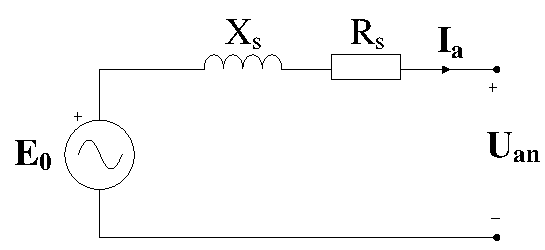
\includegraphics{EquivalentCircuit.pdf}
			\caption{Synchronous machine equivalent circuit}
			\label{fig:01}
\end{figure}
\\In order to determine the characteristics of the synchronous generator standardized tests must be carried out. The simplest method by which this is achieved are the open-circuit and the short-circuit tests. Typical open-circuit and short-circuit curves are shown in figure \ref{fig:02}. During the open-circuit the field winding is supplied with the nominal field current $I_{fn}$ and the phase voltage measured on the generator terminals is equal to $680,235\ \mathrm{V}$. In case when the field current is equal to $I_{f0} = 28 \ \mathrm{A}$, the voltage measured at the generator terminals will be equal to the nominal voltage. During the short-circuit test when the field winding current equals to $I_{f0}$ the measured stator current will be $43, 7304\ \mathrm{A}$. 
\\The per-unit system is widely used within the analysis of electrical machines. Per-unit values are obtained by dividing each parameter by a base value. For this task the base values are defined with:
\begin{itemize}
    \item peak value of the rated stator phase voltage,
    \item rated apparent power,
    \item rated angular frequency,
    \item peak value of the rated stator phase current.
\end{itemize}


\begin{figure}[!htb]
			\centering
			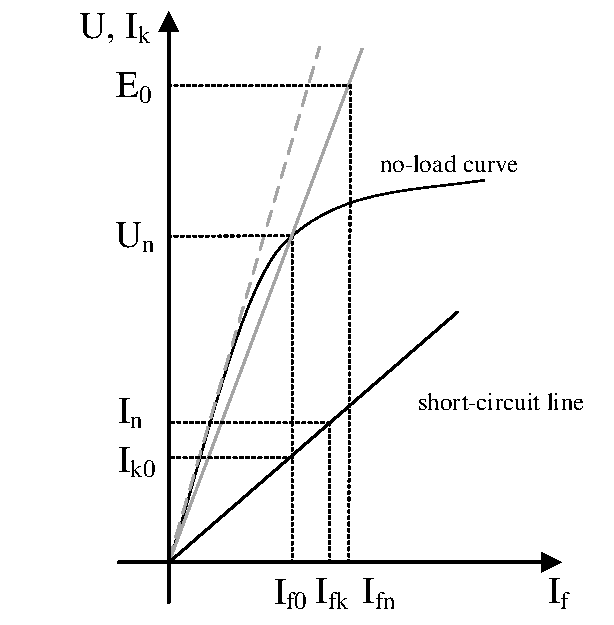
\includegraphics[scale=0.5]{NoLoadCurveShortCircuit.pdf}
			\caption{Open-circuit and short-circuit curves}
			\label{fig:02}
\end{figure}
\newpage
\subsection{Solution format and grading scheme}
Your solution must be submitted as a .csv or .xls format document with only 2 rows. The first row must consist of the required parameter names and the second row of numerical values that you calculated for each parameter. Column names must be marked as follows (columns should be in exactly this order):
\begin{itemize}
    \item stator diameter \textbf{Ds},
    \item rotor diameter \textbf{Dr},
    \item air gap length \textbf{delta},
    \item number of conductors in the stator slots \textbf{z},
    \item number of field winding turns \textbf{Nf},
    \item synchronous reactance in p.u \textbf{Xd}.
\end{itemize}
This task is graded up to 5 points. 0.5 points is given for  each correctly calculated parameter and 2 points are given for the documentation. The documentation is submitted at the end of the day. The documentation must include your calculations along with some short comments explaining the equations. You can choose the format in which the documentation will be submitted (.c script, .m script, hand written equations).  
\end{document}
